%% Version 4.3.2, 25 August 2014
%
%%%%%%%%%%%%%%%%%%%%%%%%%%%%%%%%%%%%%%%%%%%%%%%%%%%%%%%%%%%%%%%%%%%%%%
% Template.tex --  LaTeX-based template for submissions to the 
% American Meteorological Society
%
% Template developed by Amy Hendrickson, 2013, TeXnology Inc., 
% amyh@texnology.com, http://www.texnology.com
% following earlier work by Brian Papa, American Meteorological Society
%
% Email questions to latex@ametsoc.org.
%
%%%%%%%%%%%%%%%%%%%%%%%%%%%%%%%%%%%%%%%%%%%%%%%%%%%%%%%%%%%%%%%%%%%%%
% PREAMBLE
%%%%%%%%%%%%%%%%%%%%%%%%%%%%%%%%%%%%%%%%%%%%%%%%%%%%%%%%%%%%%%%%%%%%%

%% Start with one of the following:
% DOUBLE-SPACED VERSION FOR SUBMISSION TO THE AMS
%\documentclass{ametsoc}

% TWO-COLUMN JOURNAL PAGE LAYOUT---FOR AUTHOR USE ONLY
 \documentclass[twocol]{ametsoc}

%%%%%%%%%%%%%%%%%%%%%%%%%%%%%%%%
%%% To be entered only if twocol option is used

\journal{mwr}

%  Please choose a journal abbreviation to use above from the following list:
% 
%   jamc     (Journal of Applied Meteorology and Climatology)
%   jtech     (Journal of Atmospheric and Oceanic Technology)
%   jhm      (Journal of Hydrometeorology)
%   jpo     (Journal of Physical Oceanography)
%   jas      (Journal of Atmospheric Sciences)	
%   jcli      (Journal of Climate)
%   mwr      (Monthly Weather Review)
%   wcas      (Weather, Climate, and Society)
%   waf       (Weather and Forecasting)
%   bams (Bulletin of the American Meteorological Society)
%   ei    (Earth Interactions)

%%%%%%%%%%%%%%%%%%%%%%%%%%%%%%%%
%Citations should be of the form ``author year''  not ``author, year''
\bibpunct{(}{)}{;}{a}{}{,}

%%%%%%%%%%%%%%%%%%%%%%%%%%%%%%%%

%%% To be entered by author:

%% May use \\ to break lines in title:

\title{Physics-dynamics coupling with element-based high-order Galerkin methods: quasi equal-area physics grid}

%%% Enter authors' names, as you see in this example:
%%% Use \correspondingauthor{} and \thanks{Current Affiliation:...}
%%% immediately following the appropriate author.
%%%
%%% Note that the \correspondingauthor{} command is NECESSARY.
%%% The \thanks{} commands are OPTIONAL.

    %\authors{Author One\correspondingauthor{Author One, 
    % American Meteorological Society, 
    % 45 Beacon St., Boston, MA 02108.}
% and Author Two\thanks{Current affiliation: American Meteorological Society, 
    % 45 Beacon St., Boston, MA 02108.}}

\authors{Adam R. Herrington\correspondingauthor{Peter H. Lauritzen, Climate and Global Dynamics, National Center for Atmospheric Research, 1850 Table Mesa Drive, Boulder, Colorado, USA.}}

%% Follow this form:
    % \affiliation{American Meteorological Society, 
    % Boston, Massachusetts.}

\affiliation{School of Marine and Atmospheric Sciences, Stony Brook University, State University of New York, Stony Brook, New York.}

%% Follow this form:
    %\email{latex@ametsoc.org}

\email{pel@ucar.edu}

%% If appropriate, add additional authors, different affiliations:
\extraauthor{Peter H. Lauritzen}
\extraaffil{Climate and Global Dynamics, National Center for Atmospheric Research, 1850 Table Mesa Drive, Boulder, Colorado, USA.}
\extraauthor{Mark A. Taylor}
\extraaffil{Sandia National Laboratories, Albuquerque, New Mexico, USA.}
\extraauthor{Steve Goldhaber}
\extraaffil{Climate and Global Dynamics, National Center for Atmospheric Research, 1850 Table Mesa Drive, Boulder, Colorado, USA.}
\extraauthor{Kevin A. Reed}
\extraaffil{School of Marine and Atmospheric Sciences, Stony Brook University, State University of New York, Stony Brook, New York.}

%% May repeat for a additional authors/affiliations:

%\extraauthor{}
%\extraaffil{}

%%%%%%%%%%%%%%%%%%%%%%%%%%%%%%%%%%%%%%%%%%%%%%%%%%%%%%%%%%%%%%%%%%%%%
% ABSTRACT
%
% Enter your abstract here
% Abstracts should not exceed 250 words in length!
%
% For BAMS authors only: If your article requires a Capsule Summary, please place the capsule text at the end of your abstract
% and identify it as the capsule. Example: This is the end of the abstract. (Capsule Summary) This is the capsule summary. 

\abstract{Atmospheric modeling with element-based high-order Galerkin methods presents a unique challenge to the conventional physics-dynamics coupling paradigm, due to the highly irregular distribtuion of nodes within an element. The conventional coupling procedure is to evaluate the physical parameterizations (`physics') on the dynamical core grid. Evaluating the physics at the nodal points exacerbates numerical noise from the Galerkin method, enabling and amplifying local extrema at element boundaries. Grid imprinting may be substantially reduced through the introduction of an entirely separate, approximately isotropic finite-volume grid for evaluating the physics forcing. Integration of the spectral basis over the control-volumes provides an area average state to the physics, which is more representative of the state in the vicinitny of the nodal values, rather than the nodal point itself, and is more consistent with the notion of a `large-scale state' required by most physics packages. The quasi-equal area physics grid is implemented in NCAR's Community Atmosphere Model with Spectral Elements, and is shown to be effective at mitigating grid imprinting in the solution. The physics grid is also appropriate for coupling to other componenents of the Community Earth System Model, since the coupler requires component fluxes to be defined on a finite-volume grid, and one can be certain that the fluxes on the physics grid are volume-averaged fluxes.}

\begin{document}

%% Necessary!
\maketitle


%%%%%%%%%%%%%%%%%%%%%%%%%%%%%%%%%%%%%%%%%%%%%%%%%%%%%%%%%%%%%%%%%%%%%
% MAIN BODY OF PAPER
%%%%%%%%%%%%%%%%%%%%%%%%%%%%%%%%%%%%%%%%%%%%%%%%%%%%%%%%%%%%%%%%%%%%%
%

%% In all cases, if there is only one entry of this type within
%% the higher level heading, use the star form: 
%%
\section{Introduction}
An increasing number of numerical methods publications in the atmospheric science literature concern transport, shallow-water, and three-dimensional models employing element-based high-order Galerkin discretizations such as finite-element and discontinuous Galerkin methods \citep[for an introduction to these methods see, e.g., ][]{Durran,NLL2011LNCSE}. Some global models based on Galerkin methods have reached a level of maturity for which they are being considered for next generation climate and weather models due to their inherent conservation properties, high-order accuracy (for smooth problems), high parallel efficiency, high processor efficiency, and geometric flexibility facilitating mesh-refinement applications. NCAR's Community Atmosphere Model \citep[CAM; ][]{CAM5} offers a dynamical core based on continuous Galerkin finite elements \citep{TF2010JCP}, referred to as CAM-SE \citep[CAM Spectral Elements; ][]{DetAl2012IJHPCA,TES2008JPCS,LetAl2017MWR}. CAM-SE is, in particular, being used for high resolution climate modeling \citep[e.g., ][]{JAME:JAME20125,BetAl2013JC,RetAl2015GRL} and static mesh-refinement applications \citep[e.g., ][]{FT2004MWR,ZetAl2014JC,ZetAl2014JCb,GetAl2014GMD,RHUZ2016JAMC}. Other examples of models based on high-order Galerkin methods that are being considered for `operational' weather-climate applications are \citet{Giraldo20083849}, \citet{NCT2009CF} and \citet{BSBDK2013TCFD}.

\begin{figure}[t]
\noindent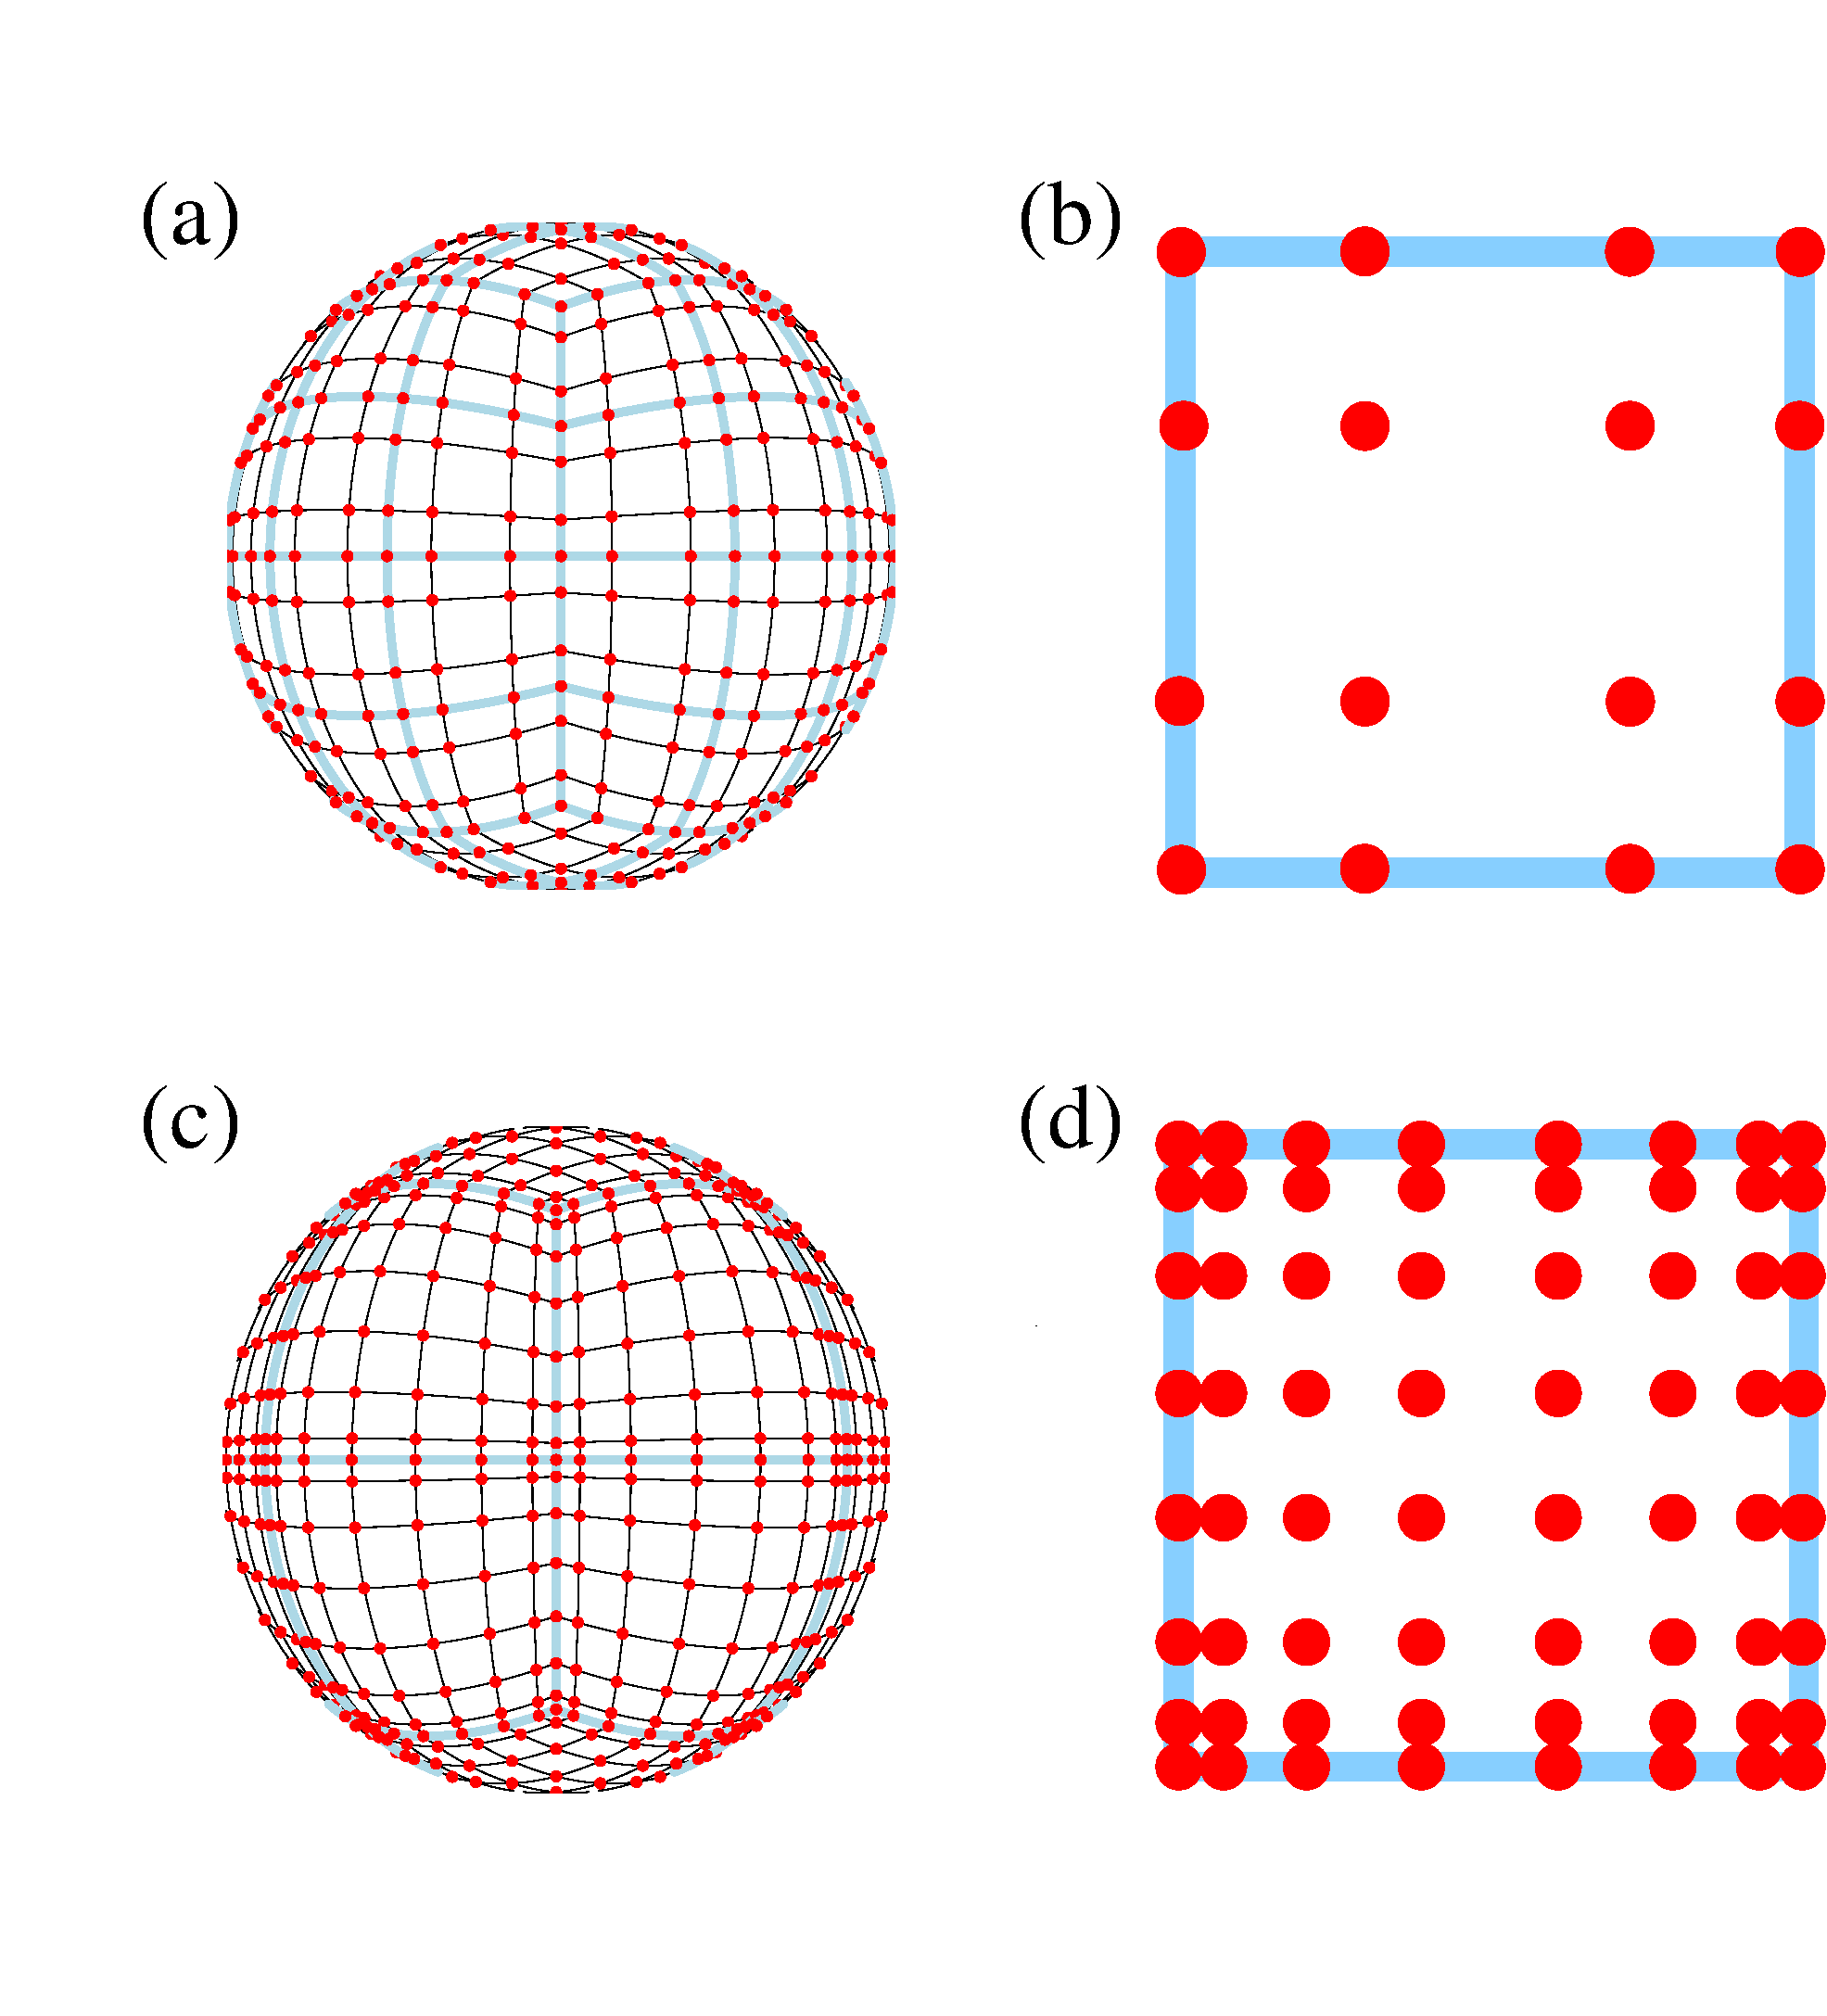
\includegraphics[width=19pc,angle=0]{figs/quadrature-fig/gll.pdf}\\
\caption{Example of CAM-SE GLL quadrature grids, marked with red filled circles, (a \& c) on the cubed-sphere and (b \& d) in an element. (a)-(b) and (c)-(d) use $4\times 4$ ($np=4$) and $8\times 8$ ($np=8$) GLL quadrature points in each element, respectively. (a) and (c) have the same average grid-spacing at the Equator (7.5$^\circ$) which is obtained by using (a) $4\times 4$ ($ne=4$) and (b) $2\times 2$ ($ne=2$) elements on each cubed-sphere face/panel, respectively. The element boundaries are marked with thick light blue lines. The grid configurations shown on (a) and (c) are referred to as $ne4np4$ and $ne2np8$, respectively.}
\label{fig:gll-grids}
\end{figure}

Assumptions inherent to the physical parameterizations (also referred to as {\em{physics}}) require the state passed by the dynamical core to represent a `large-scale state', for example, in quasi-equilibrium-type convection schemes \citep{AS1974JAS,PC2008JAS}. In finite-volme methods, one may think of the dynamical core state as the average state of the atmosphere over a control volume, and for resolutions typical of climate simulations is entirely consistent with the notion of a `large-scale state'. For finite-difference methods the point value is thought of as representative for the atmospheric state in the vicinity of the point value and one can usually associate a volume with the grid-point. Hence the physics grid (the grid on which the state of the atmosphere is evaluated and passed to physics) and the dynamics grid (the grid the dynamical core uses) coincide. Having the physics and dynamics grids coincide is obviously convenient since no interpolation is needed (which could disrupt conservation properties) and the number of degrees of freedom on both grids is exactly the same. 

For the regular latitude-longitude, cubed-sphere and icosahedral grids the distance between the grid-points is gradually varying for finite-volume/finite-difference discretizations. For high-order element-based Galerkin methods, the dynamical core grid is defined by the quadrature points. For the case of CAM-SE these are the Gauss-Lobatto-Legendre (GLL) quadrature points. A unique aspect of the high-order quadrature rules is that the nodes within an element are not equally spaced. For example, Figure \ref{fig:gll-grids} shows GLL points on an individual element of a cubed-sphere grid for degree 3 ($np=4$ quadrature points) and degree 7 ($np=8$ quadrature points) polynomial basis in CAM-SE. Both grids have the same average resolution on the sphere (due to different number of elements), however, the higher the order of the quadrature rule the less equi-distant are the quadrature points. GLL quadrature points cluster near the edges and, in particular, the corners of the elements.

\begin{figure}[t]
\noindent\includegraphics[width=19pc,angle=0]{figs/se_gll_cv_grid.eps}\\
\caption{An example of control volumes constructed around GLL quadrature points (NE4NP4) so that the spherical area of the control volumes exactly match the quadrature weight multiplied by the metric factor.}
\label{fig:cv-grids}
\end{figure}

If the conventional physics-dynamics coupling paradign is applied to CAM-SE, then the physics are evaluated at the GLL nodes, and a volume associated with the quadrature point should be defined. An example of that is shown on Figure \ref{fig:cv-grids} where control volumes have been defined around the quadrature points so that the spherical area of the control volumes exactly match the Gaussian weight multiplied by the metric term (these weights are used for integrating the basis functions over the elements and can therefore, in this context, be interpreted as areas). [{\color{red}{Mark: could we be mathematically more rigorous? perhaps an appendix describing the iterative algorithm?}}] This grid is used in the NCAR CESM (Community Earth System Model) coupler for passing states between ocean, atmosphere and land components since the current remapping method is finite-volume based and therefore requires control volumes {\footnote{it is noted that methods exist that do not require control volumes for conservative interpolation \citep{UT2015MWR}}}. Hence the components `see' an irregular atmospheric grid. Similarly, the parameterizations in the atmosphere `see' a state that is anisotropically sampled in space \citep[see Figure 1 and 5 in ][]{KetAl2008JGR}.% Physical inconsistencies may arise, for example, if assumptions inherent to the physics break down only at the smallest control volumes on the grid.

It would be incorrect to interpet the irregular size of control volumes in Figure~\ref{fig:cv-grids} as an equivalent spread in the scales of motion resolved by the dynamical core. The scales of motion are defined by the degree of the Lagrange basis in each element, and the nodes may be viewed as irregularly spaced samples of an underlying spectrally truncated state. From this perspective, one might expect the solution to be independent of control volume size. An aqua-planet simulation \citep{NH2000ASL,MWO2016JAMES} is carried out using CAM-SE (Figure~\ref{fig:omega-se-volumes}), and the probability density distribution of the upward vertical pressure velocity ($\omega$), conditionally sampled based on three categories - `interior nodes', with their large grid cell areas, and `edge' and `corner' nodes with their characteristically smaller grid cell areas - is shown in Figure \ref{fig:omega-se-volumes}. Their is an apparent dependence on control volume size, with interior nodes being characteristically sluggish and intially at odds with the expectation. However, the lack of a distinction between `corner' and `edge' solutions is consistent with our expectation. It turns out, that `corner' and `edge' solutions are similar because they have something else in common - they both lie on an element boundary. The division of solutions shown in Figure~\ref{fig:omega-se-volumes} is primiarily between whether a node is, or is not situated on an element boundary, and is a nuanced signature of high-order element-based Galerkin methods for non-smooth problems.

\begin{figure}[t]
\noindent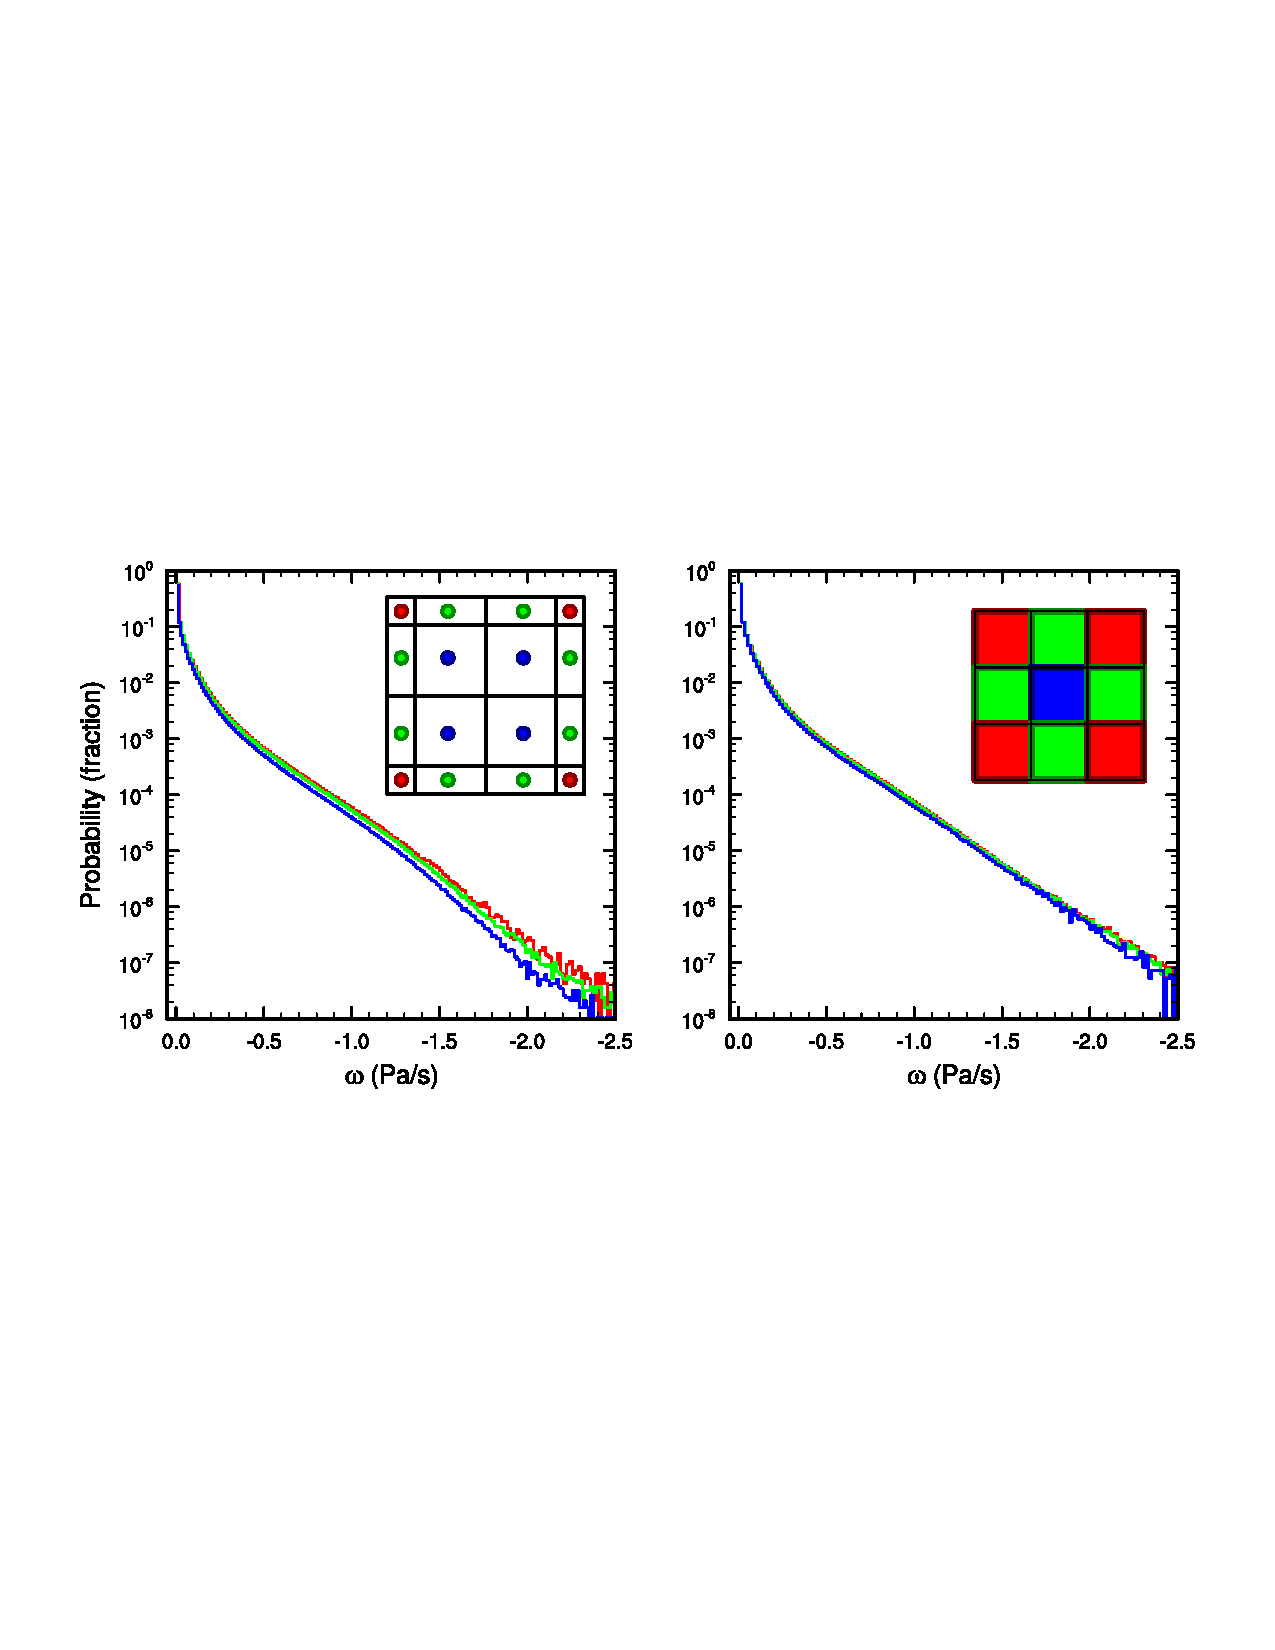
\includegraphics[width=19pc,angle=0]{figs/temp_pdf_omg_np4_v_pg3_CROP.pdf}\\
\caption{Probability density distribution of instantaneous upward $\omega$ in a pair of aqua-planet simulations using CAM4 physics. Figure is constructed from one year of six hourly data, at all vertical levels. (Left) $ne30np4$ configuration conditionally sampled for interior, edge and corner node control volumes, and (Right) $ne30pg3$ configuration, but sampled by within-element physics grid-cell location. Note the consistently larger magnitude $\omega$ for boundary nodes compared with interior nodes, and that the bias is eliminated through mapping to a quasi-equal area physics grid.}\label{fig:omega-se-volumes}
\end{figure}

The quadrature grid in element-based Galerkin methods is defined to perform mathematical operations on the basis functions, e.g., computing gradients and integrals, rather than evaluating the state variables for physics-dynamics coupling. While the interior quadrature nodes are high-order $C^{\infty}$ in CAM-SE, the smoothness of boundary nodes are constrained by the need to patch neighboring solutions together to form a globally continuous solution, known as the direct stiffness summation (DSS). The DSS operation is attractive because it allows for high-order accuracy with minimial communication between elements, but results in a $C^0$ degradation at element boundaries (Figure~\ref{fig:se-schematic}). Through evaluating the physics at the nodal points, strong grid-scale forcing or oscillatory behavior near an element boundary may exacerbate the discontinuity (Figure~\ref{fig:se-schematic}). The greater magnitude vertical motion of boundary nodes in Figure~\ref{fig:omega-se-volumes} is therefore due to the systematically tighter pressure gradients on element boundaries. One may argue that it would be more consistent to integrate the basis functions over quasi-equal area control volumes within each element and pass those control volume average values to physics rather than irregularly spaced quadrature point values. In this case when integrating basis functions over control volumes a grid-cell average value is more representative of the values near the extrema at the element boundary than the quadrature point value. The relationship between the nodal values, the basis functions and the proposed control volumes is illustrated schematically in one-dimension in Figure \ref{fig:physgrid-1d}. 

\begin{figure*}[t]
\noindent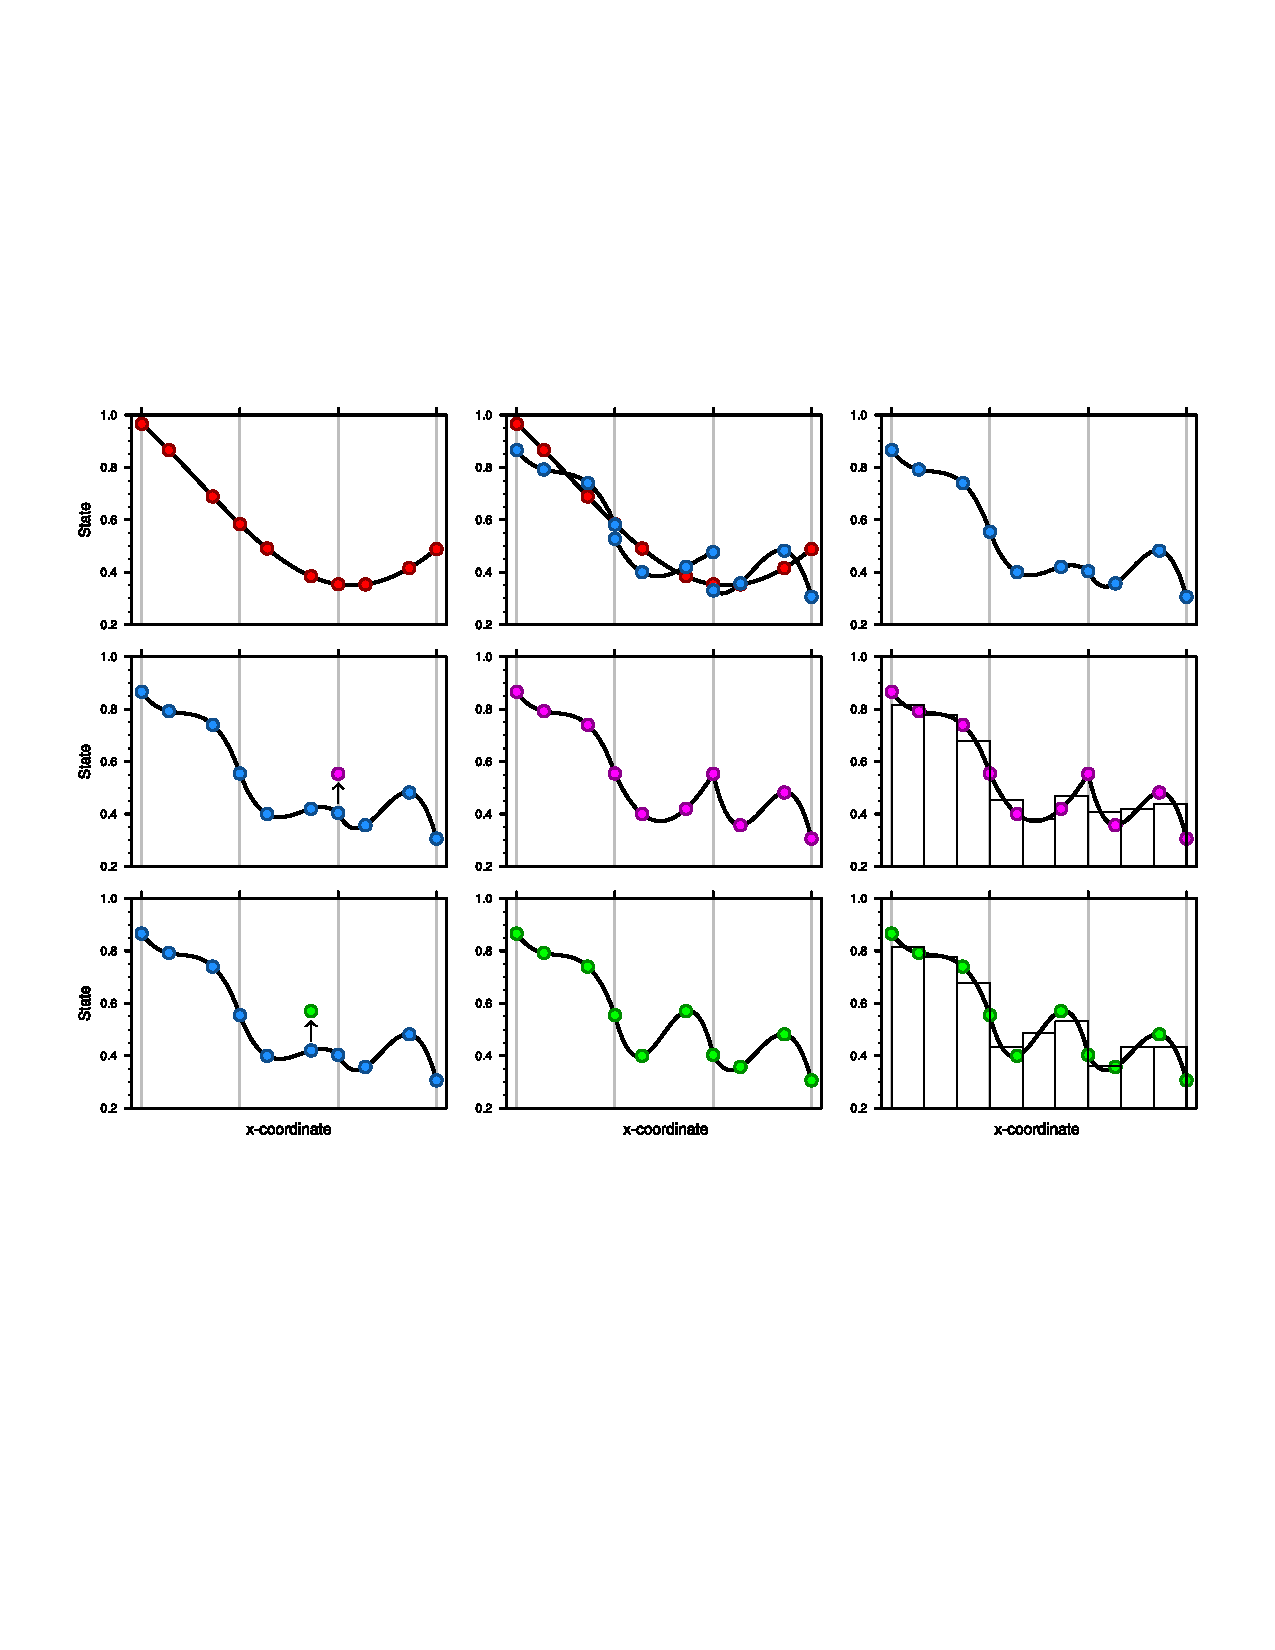
\includegraphics[width=38pc,angle=0]{figs/se-schematic-arh.pdf}\\
\caption{A 1D schematic illustration on how CAM-SE advances the solution to the equations of motion in time. Consider 3 elements. The red filled circles are the GLL quadrature points in each element ($np=4$). Note that the quadrature points on the boundary are shared between elements. (a) Assume a degree 3 global Lagrange polynomial initial condition (red curve) which can be represented exactly by the degree 3 Lagrange basis in each element. (b) The solution to the equations of motion are advanced in time (one Runga-Kutta step) independently in each element leading to the quadrature values marked with filled purple circles. The Lagrange basis is shown with red curves connecting the purple circles. There are now two solutions, one from left and one from right, for the quadrature points at the element end points. In CAM-SE the values are averaged so that the solution is $C^0$. Note that the averaging changes the Lagrange polynomials throughout except at the internal quadrature points. (c) shows the solution after averaging. (d) Assume there is a grid-scale forcing that increases the quadrature value located at $x=3$. (e) The solution is now clearly $C^0$ at the element boundary at $x=3$. (f) Histogram shows the average values resulting in integrating the basis functions over the control volumes.}
\label{fig:se-schematic}
\end{figure*}

\begin{figure*}[t]
\noindent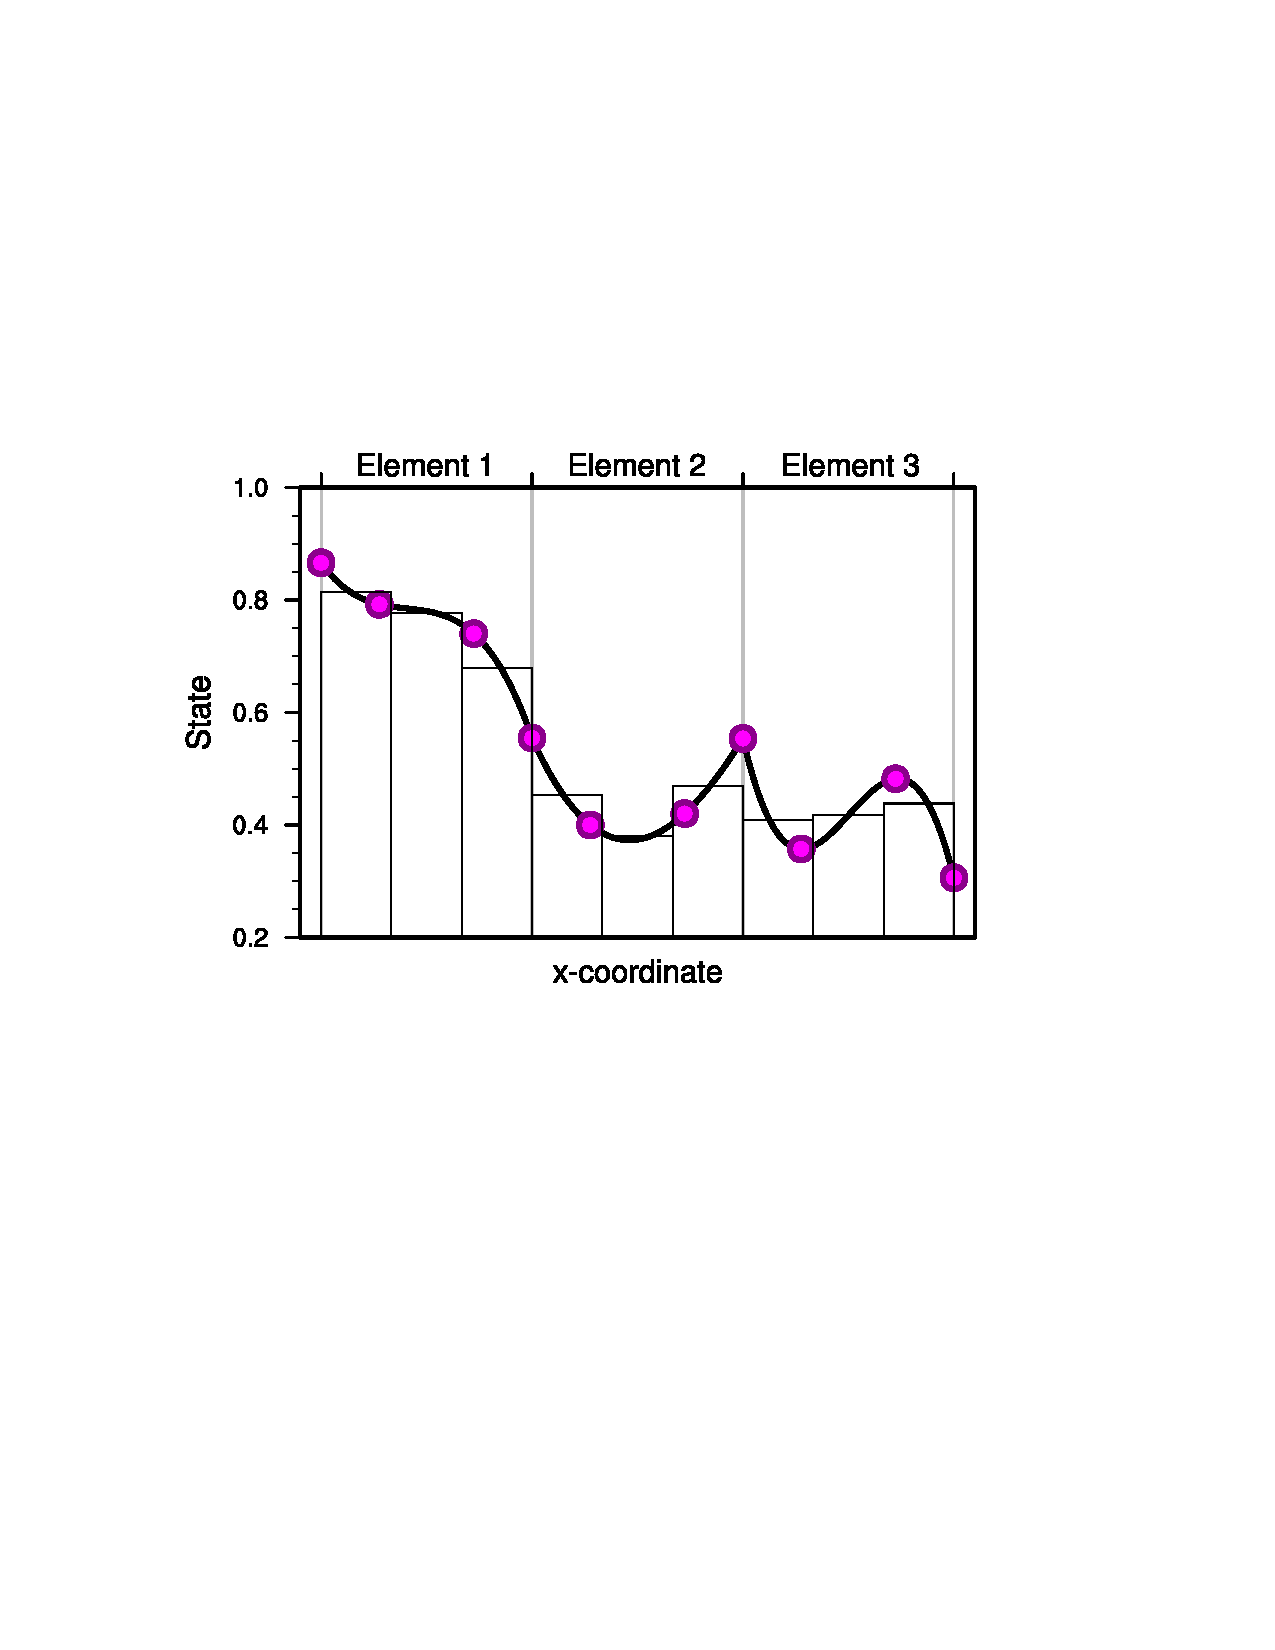
\includegraphics[width=38pc,angle=0]{figs/physgrid-1d_3x3-arh.pdf}\\
\caption{A graphical illustration of the physics grid in one dimension. Three elements are shown and the filled red circles are the GLL quadrature points in each element. The red curve is the basis function representation of the field and the green filled circles are the quadrature point values. The physics grid divides each element into 3 equal-area control volumes. The histogram shows the average values over the physics grid control volumes resulting from integrating the basis functions over the respective control volumes.}
\label{fig:physgrid-1d}
\end{figure*}


It is the purpose of this paper to document the design of CAM-SE with an approximately isotropic physics grid, in which the physics and dynamics grids are entirely separated as illustrated in one dimension in Figure~\ref{fig:physgrid-1d}. The mapping procedures used in the physics grid configuration are presented in Section 2. Idealized model configurations with and without topography are presented in Section 3, illustrating a marked reduction in grid imprinting due to the use of a quasi-equal area physics grid. Section 4 contains a discussion of results and concluding remarks. 

\section{Methods}
Here we focus on CAM-SE, however, in principle the methods apply to any element-based high-order Galerkin model. The physics grid in CAM-SE is defined by sub-dividing each element using equi-angular gnomonic coordinate lines to define the sides of the physics grid control volumes. Note that the element boundaries are defined by equi-angular gnomonic grid lines. The notation $pg=3$ refers to the configuration where the elements are divided into $pg\times pg=3\times 3$ quasi equal-area physics grid cells (see Figure \ref{fig:np4_pg3}). Defining the physics grid by sub-diving elements makes it possible to use the same infrastructure as used for the quadrature point values thereby facilitating its implementation in CAM-SE. Here we make use of the $ne30np4$ and $ne30pg3$ grids that use GLL quadrature point physics grid (physics and dynamics grid coincide), and the same ($pg=3$) resolution quasi equal-area physics grids, respectively. In all configurations we use degree 3 Lagrange basis ($np=4$) and $ne\times ne=30\times 30$ elements on each cubed-sphere panel resulting in an average GLL quadrature point spacing at the Equator of $1^\circ$. %Vertical grid spacing is the standard CAM5 configuration ($nlev=30$)

The separation of grids was made possible through the implementation of the Conservative Semi-Lagrangian Multi-tracer transport scheme in CAM-SE (CAM-SE-CSLAM;\cite{}). Tracers evolve in CSLAM using a semi-lagrangian method on the finite-volume grid (Figure~\ref{fig:physgrid-1d}). The physics grid configuration ($pg=3$) is distinct from CAM-SE in that it not only has a finite-volume physics grid, but that the tracers evolve on the finite-volume grid using CSLAM. For this reason, the physics grid configuration is referred to as CAM-SE-CSLAM throughout the study.

\begin{figure*}[t]
\noindent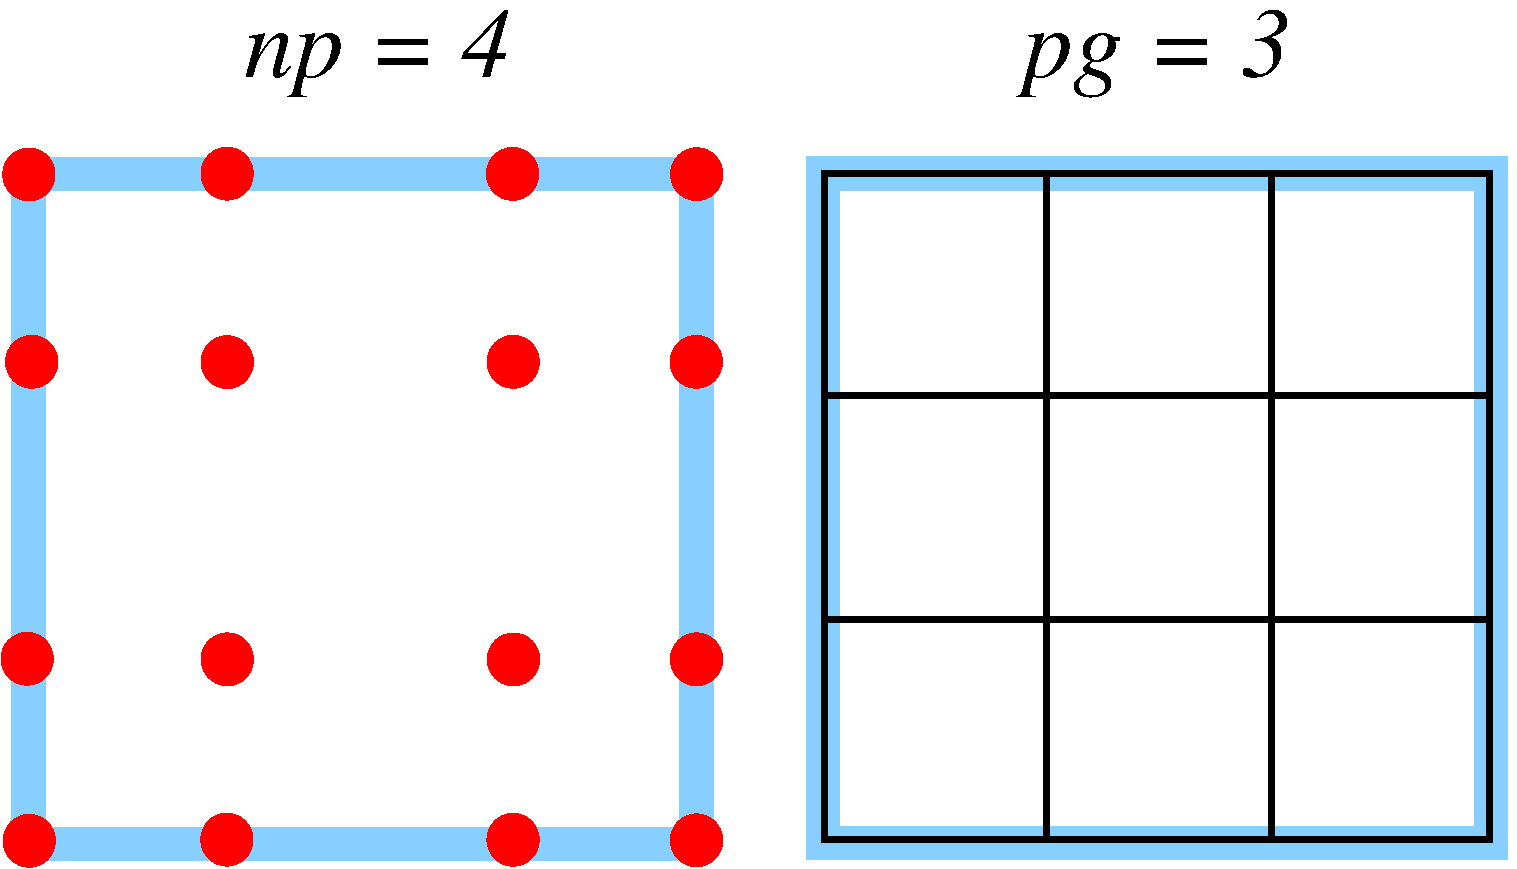
\includegraphics[width=38pc,angle=0]{figs/np4_pg3.pdf}\\
\caption{A schematic illustration of an element, indicating the relationship between (left) the dynamical core grid, and (right) the proposed quasi-equal area physics grid. The phyiscs grid contains $pg x pg$ grid cells in each element, and $pg = 3$.}
\label{fig:np4_pg3}
\end{figure*}


A consequence of separating physics and dynamics grids is that the atmospheric state must be mapped to the physics grid and the physics tendencies must be mapped back to the dynamics grid which is discussed in separate sections below. 
\subsection{Mapping state dynamics grid (GLL) to physics grid (physgrid)}
The dynamics state is defined on the GLL grid in terms of temperature $T^{(gll)}$, zonal wind component $u^{(gll)}$, meridional wind component $v^{(gll)}$, and dry pressure level thickness $\Delta p^{(gll)}$. In the mapping of the atmospheric state to the physics grid it is important that the following properties are met:
\begin{enumerate}
\item conservation of scalar quantities such as mass and thermal energy,\label{prop1}
\item for tracers; shape-preservation (monotonicity), i.e. the mapping method must not introduce new extrema in the interpolated field, in particular, negatives,\label{prop2}
\item consistency, i.e. the mapping preserves a constant,\label{prop3}
\item linear correlation preservation.
\end{enumerate}
Other properties that may be important, but not pursued here, is total energy conservation and axial angular momentum conservation. We argue that the most consistent method for mapping scalar state variables from the GLL grid to the physics grid is to integrate the Lagrange basis functions representation (used by the SE dynamical core) over the physics grid control volumes, i.e. integrate the basis function representation of $\Delta p^{(gll)}\times T^{(gll)}$ and $\Delta p^{(gll)}$ over the physics grid control volume \citep[see, e.g., ][]{LTOUNGK2017MWR,UT2015MWR}{\color{red}{add Appendix with details}}. Thermal energy and dry air mass is conserved and the mapping is consistent. For the wind, which is a vector, the latitude-longitude wind components are mapped by transforming to contra-variant wind components, evaluate the basis function representation thereof at the equi-angular center of the physics grid control volumes and then transform back to latitude-longitude coordinate system winds. 

The mapping of tracers is more problematic since the basis function representation is oscillatory although the shape-preserving filter guarantees shape-preservation at the GLL nodes \citep{GTS2014JCP}. To avoid this issue we use the CAM-SE-CSLAM version of CAM-SE where tracers are advected on the 3x3 physics grid. Note that in CAM-SE-CSLAM the dry mass internally predicted by CSLAM, $\Delta p^{(cslam)}$, is, by design, equal to $\Delta p^{(gll)}$ integrated over the CSLAM/physics grid control volume \citep{LTOUNGK2017MWR}. Since the tracer grid and physics grids are co-located and $\Delta p^{(physgrid)}=\Delta p^{(cslam)}$ then the  mass conservation, correlation preservation, consistency and shape-preservation constraints are trivially fulfilled.

\subsection{Mapping tendencies from physics grid (physgrid) to dynamics grid (GLL)}
The physics tendencies are computed on the finite-volume physics grid and are denoted $f_T^{(phys)}$,$f_u^{(phys)}$,$f_v^{(phys)}$, and $f_m^{(phys)}$. Note that dry air mass is not modified by physics and hence there is no tendency for dry mass,  $f_{\Delta p}\equiv 0$. Also, it is important to map tendencies and not state from the physics grid to GLL grid otherwise one will get spurious tendencies from mapping errors when the actual physics tendency is zero (unless a reversible map is used).

It is important that this process:
\begin{enumerate}
\item preserves a zero tendency,
\item for tracers; mass tendency is conserved,
\item for tracers; in each tracer grid cell the mass tendency from physics must not exceed tracer mass available in tracer grid cell (it is assumed that the physics tendency will not drive tracer mixing ratio negative on the physics grid),\label{item:phys2fvm_consistency}
\item linear correlation preservation,
\item consistency, i.e. the mapping preserves a constant.
\end{enumerate}
Other properties that may be important, but not pursued here, is total energy conservation (incl. components of total energy) and axial angular momentum conservation. Scalar variables are mapped from physics grid to GLL grid using a tensor-product Lagrange interpolation. The local coordinates on a cubed-sphere are discontinuous at the element edges so the interpolation requires special attention at the cube corners and edges. The details are provided in Appendix \ref{appendix}. Lagrange interpolation preserves a constant (including zero) and linear correlations. Tracer and physics grids are co-located so tracer mass, tracer shape, and tracer correlations are trivially preserved on the tracer grid; and the inconsistency in point \ref{item:phys2fvm_consistency} above will not appear. We do, however, need to map water tracers to the GLL grid to account for moist effects in the equations of motion. The CSLAM water tracer mixing ratios updated by physics tendencies are mapped to the GLL grid using the same tensor cubic interpolation as is used for temperature and velocity components. In between the calls to physics (i.e. in the dynamical core sub-stepping) the water tracers are advected on the GLL grid with the SE method.



\begin{itemize}
\item {\color{red}{mention why we are not doing cslam-like mapping; mention why we are not using Paul's algorithm}}
\item {\color{red}{in results section we might want to show some energy diagnostics and estimate PDC errors; must be run with $cp_{dry}$}}
\end{itemize}





\section{Results}

The CAM aqua-planet reference configuration \citep{NH2000ASL,MWO2016JAMES} consists of an ocean covered planet in a perpetual equinox, with fixed, zonally symmetric SST temperatures idealized after the present day climatology. Two year long aqua-planet simulations are performed, using CAM-SE in the $ne30np4$ default configuration, and with the $ne30pg3$ physics grid configuration. A plot similar to Figure \ref{fig:omega-se-volumes} is constructed for the $ne30pg3$ simulation, in which a probability density distribution of upward $omega$ in the deep tropics is conditionally sampled based on location within the element. In the $ne30pg3$ configuration, the sampling is based on a grid cell index 1-9, corresponding to the control volume location within the element (Figure \ref{fig:omega-se-volumes}). Through the use of the physics grid, the dynamical state appears independent of location within the element, a marked improvement over the $ne30np4$ (Figure \ref{fig:omega-se-volumes}). Since the state is independent of in-element location, it follows that the physics forcing, which is evaluted from the state, should also be independent of within-element location. The low-level, mean and variance of the physics tendencies in the two aqua-planet simulations are shown in Figure \ref{fig:tendency_imprint}. The mean physics tendencies contains modest grid imprinting in the default configuration, while in the variance field, grid imprinting is both ubiquitous and unmistakable (Figure~\ref{fig:tendency_imprint}). The variance is larger on boundary nodes (Figure~\ref{fig:tendency_imprint}), reuslting in a clear `stitching' pattern resembling the cube-sphere grid. In $ne30pg3$, the grid imprinting is all but eliminated based on the mean and variance of the physics tendencies (Figure~\ref{fig:tendency_imprint}).

\begin{figure}[t]
\noindent\includegraphics[width=19pc,angle=0]{figs/QPC6_bar_skk.pdf}\\
\caption{Mean (left) and variance (right) of the low level temperature tendencies from the physical parameterizations on the GLL grid, with the $ne30np4$ configuration, top row) and $ne30pg3$ configuration (bottom row), in a pair of year-long aqua-planet simulations after \cite{MWO2016JAMES}. Grid imprinting is observed along the element boundaries in $ne30np4$, but is absent from the $ne30pg3$ simulation.}
\label{fig:tendency_imprint}
\end{figure}

Grid imprinting associated with the flow around obstacles is more problematic than that encountered on the aqua-planets. In order to diagnose grid imprinting associated with topographic flow, an idealized held-suarez conifugration \citep{HS1994} is outfitted with real world topography, and ran for a year using the $ne30np4$ and $ne30pg3$ configurations. Figure~\ref{fig:FHS-contours} shows the mean $\omega$ at two different vertical levels in the middle troposphere. At higher latitudes (such as southern Andes), the flow is smooth, conforming reasonably to the underlying topography. At lower latitudes, over the Andes or the Himlayas, their is a clear preferance for larger magnitude vertical motion to occur at the element boundaries. The vertical structure of $\omega$ in regions of strong grid-imprinting is depicted in Figure~\ref{fig:FHS-transect}, which are great-circle distance-pressure transects over the Andes and Himalayas. The $\omega$ field indicates large magnitude upward motion occurs as the flow approaches the foot of a topographic obstacle. Compensating downward motion tends to occur about 2 GLL nodes downwind of the strong upward motion (although sometimes they form up-slope). The full troposphere upward-downwawrd couplets are an indication that grid imprinting due to topography is enhanced in regions of weak stratificaiton, such as occurs in the deep tropics, with forced upslope flow facilitating the release of gravitational instabilty. The greater magnitude vertical motion is a result of the characteristically tighter pressure gradients at element boundaries. 

\begin{figure}[t]
\noindent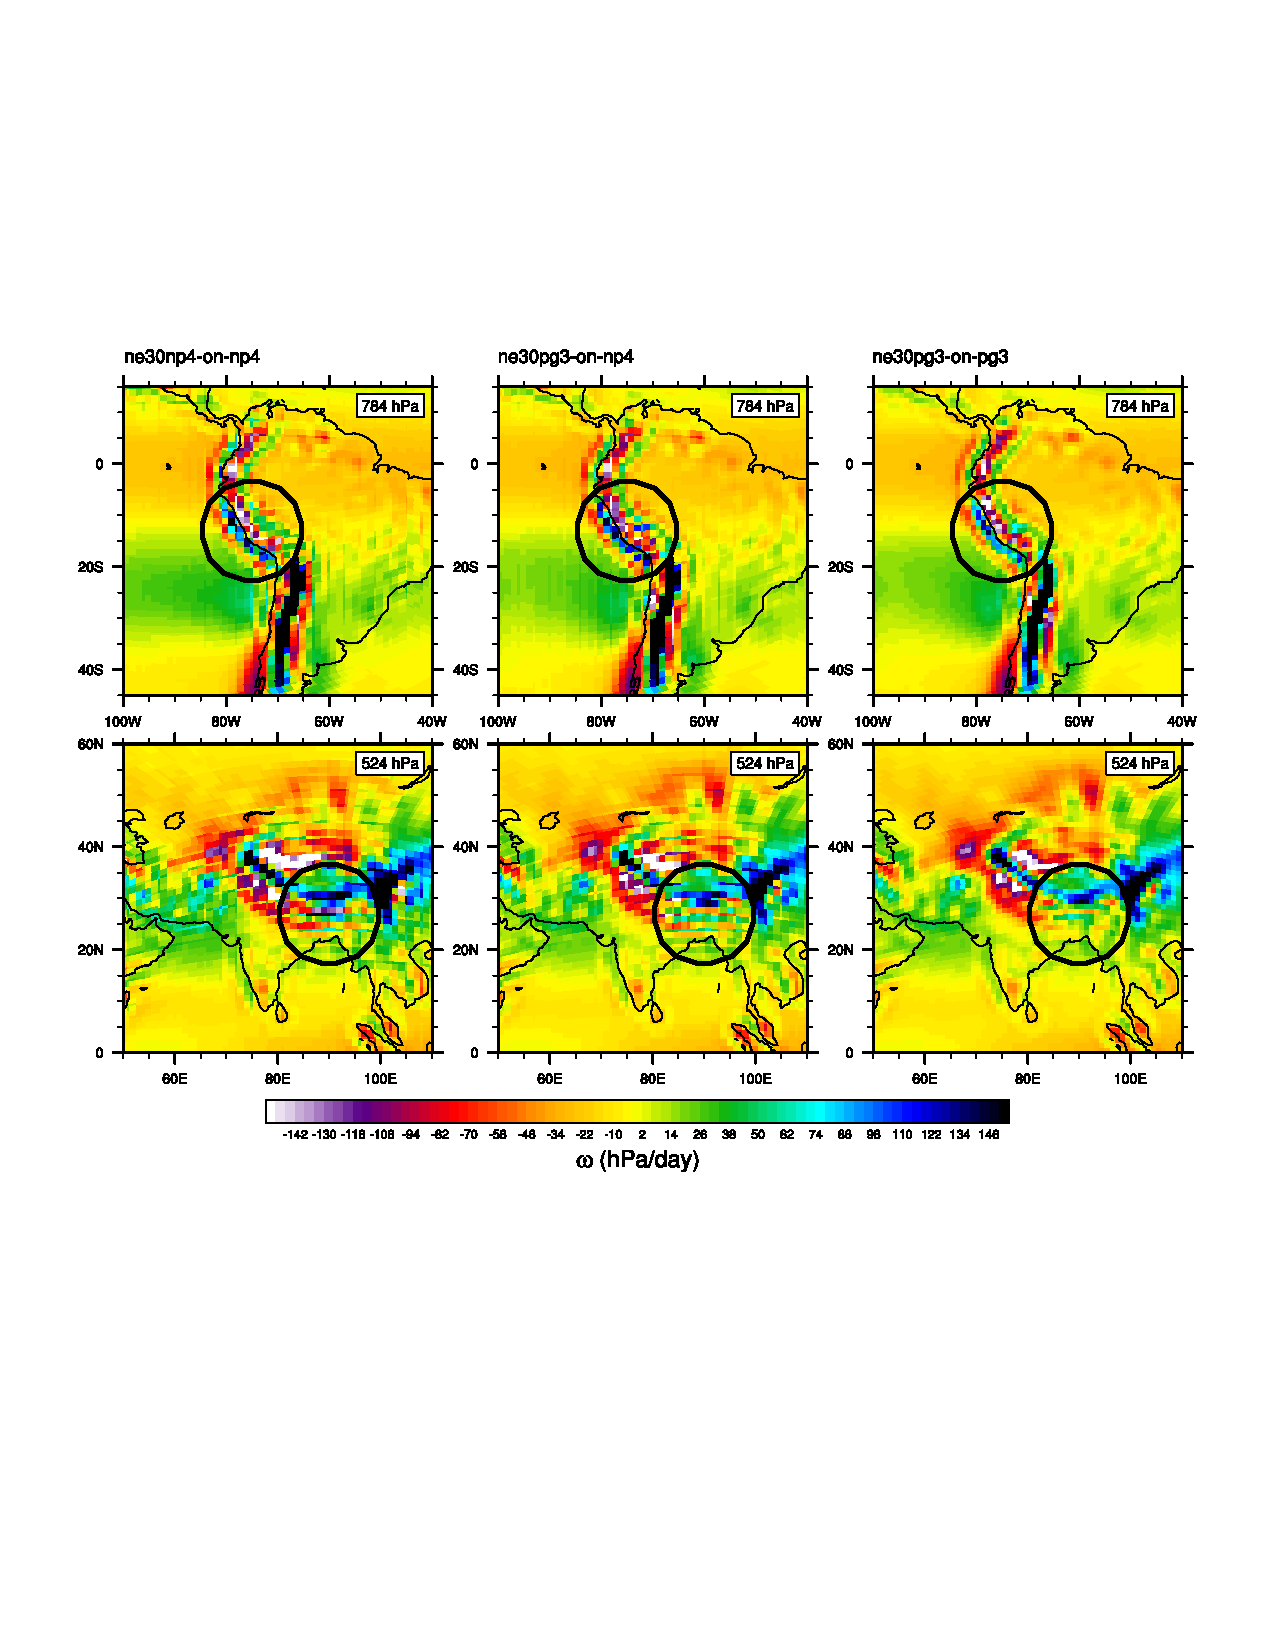
\includegraphics[width=19pc,angle=0]{figs/FHS-contours-CROP.pdf}\\
\caption{Mean $\omega$ at two model levels in the middle troposphere, in a Held-Suarez configuration outfitted with real world topography. (Left) CAM-SE state on the GLL grid, $ne30np4$, (Middle) CAM-SE-CSLAM state on the GLL grid, $ne30np4$ and (Right) CAM-SE-CSLAM state on the physics grid, $ne30pg3$. The $\omega$ fields are computed from a 1200 day Held-Suarez simulation. White lines denote the great circle transects in \ref{fig:FHS-transect}.}
\label{fig:FHS-contours}
\end{figure}


%The grid-imprinting tends to be exaggerated in the modified held-suarez configuration, compared to more realistic configurations using a complete physical parameterization package. Figure~\ref{fig:FHS-contours} depicts the $omega$ field in an AMIP simulation, which contains less grid imprinting compared to the Held-Suarez configuration through the use of the CAM6 physics pacakge \citep{}. Physics packages contain convection schemes, whose purpose is to remove gravitational instabilites through subgrid-scale vetical mixing. Since the idealized Held-Suarez physics does not contain a convection scheme, the dynamical core tends to be more active in removing gravitational instability, compared to a full physics configuration. Note that the implications of this finding are that one can accept a level of grid-impriniting in the modified Held-Suarez configuration, and trust that it will be absent in more real-world configurations.

\begin{figure}[t]
\noindent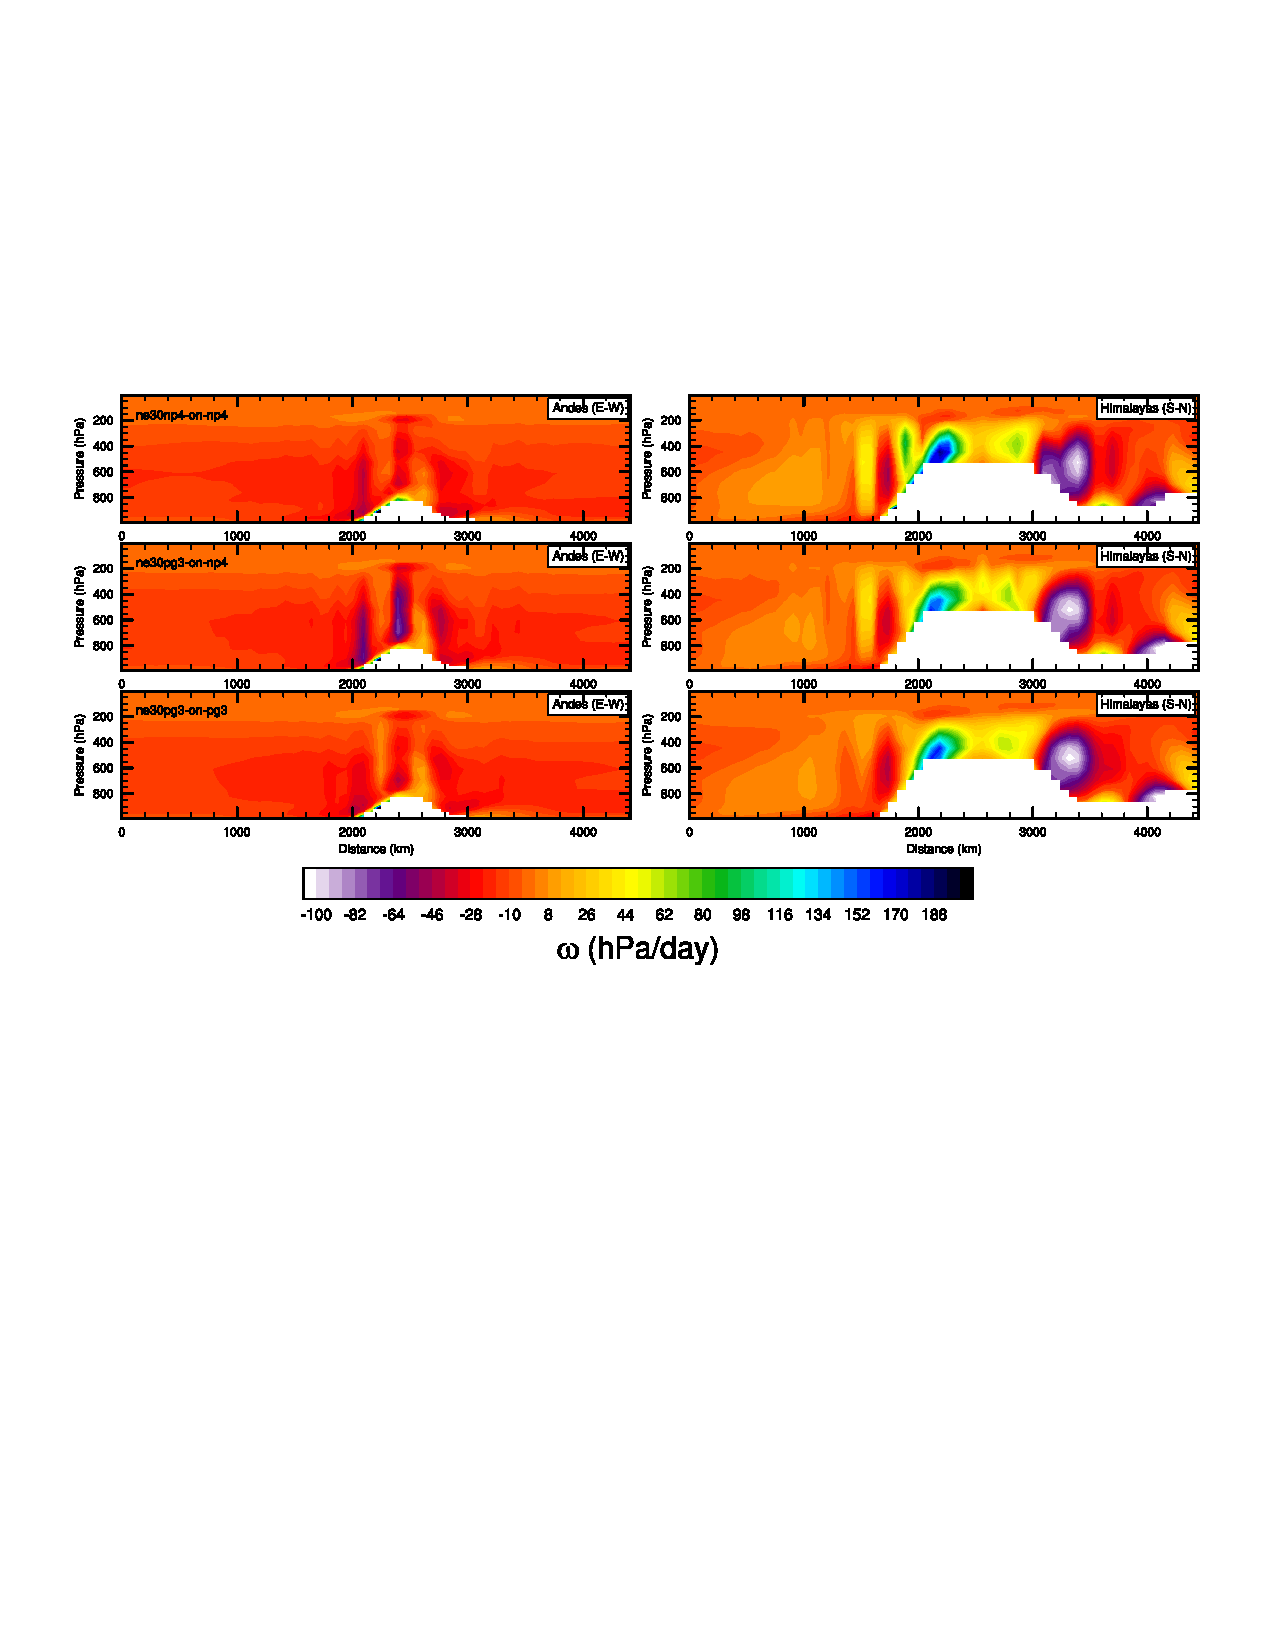
\includegraphics[width=19pc,angle=0]{figs/FHS-transect-CROP.pdf}\\
\caption{Great circle distance-pressure transect of $omega$ in the Held-Suarez simulations with realistic topography. $omega$ field derived from the final 12 months of a 13 month simulation.}
\label{fig:FHS-transect}
\end{figure}

Through the use of the physics grid, grid imprinting due to topographic flow is reduced (Figures~\ref{fig:FHS-contours} and \ref{fig:FHS-transect}). Figures~\ref{fig:FHS-contours} and \ref{fig:FHS-transect} also show the state in CAM-SE-CSLAM, but on the dynaimcal core grid. Arguably, the grid imprinting due to topography in CAM-SE-CSLAM, is not much of an improvment from CAM-SE, from the perspective of the dynamical core grid. The CAM-SE-CSLAM solution does have less grid imprinting, over the Andes and Himalayas, from the perspective of the physics grid. The reduction in grid imprinting is almost entirely a result of the smoothing effect of integrating the basis functions over the control volumes in the physics grid. The native topography lives on the physics grid, and the surface geopotential is mapped to the nodal points at run-time in $ne30pg3$. The mapping method does not introduce new extreme to the nodal points, and the topography tends to be smoother at the element boundaries, relative to $ne30np4$. This effect is rather small, with differences between CAM-SE and CAM-SE-CSLAM topography on the order of a few meters. In regions of gravitational instability, the flow appears damped compared to the $ne30np4$ configuration, even from the perspective of the dynamics grid (Figure~\ref{fig:FHS-transect}). We speculate that this damped motion may result from the use of a slightly smoother topography, as viewed by the dynamical core grid.  

% \subsection{First secondary heading}

% \subsubsection{First tertiary heading}

% \paragraph{First quaternary heading}


\section{Conclusions}

Element-based high-order Galerkin Methods possess many of the attractive qualitites recommended for next generation global atmopsheric models. Among these, high-order accuracy is acheived with minimal communication between elements, allowing for near perfect scaling on massively parallel systems. Element communication amounts to a numerical flux applied to the element boundaries, reconciling overlapping solutions of adjacent elements but degrading the order of accuracy of the boundary nodes in the process (to $C^0$). For non-smooth problems, gradients are systematically tighter at the element boundaries, and local extrema often characerize the boundary nodes. This behavior is illustrated using NCAR's Community Atmosphere Model with Spectral Elements dynamics (CAM-SE) in an aqua-planet configuration, and in a Held-Suarez configuration with real-world topography. 

The authors argue that the conventional physics-dynamics coupling paradigm, in which the physical parameterizations are evaluated on the dynamical core grid, exacerbates grid imprinting by commuting boundary node extrema through the physics forcing. A separate physics grid is proposed and implemented in CAM-SE, and referred to as CAM-SE-CSLAM, through dividing the elements into quasi-equal areas with equivalent degrees of freedom. The state is mapped to the physics grid with high-order accuracy through integrating CAM-SE's Lagrange basis functions over the control volumes. Control volumes near element boundaries now represent a state in the vicinity of the extrema produced through the boundary exchange operation, as opposed to the the nodal value itself. The physical parameterizations are evaluated on the finite volume grid, and the forcing terms are mapped back to the dynamical core grid {\color{red}{discuss mapping back}}. In aqua-planet simulations, evaluating the paramterizations on the physics grid removes any obvious dependence of proximity to the element boundary, resulting in a more realistic state with negligeable grid imprinting.

In CAM-SE-CSLAM, the physics grid replaces the finite-volume grid used to compute fluxes between model components in CAM-SE (Figure~\ref{fig:}). The appeal here is two-fold. Through integrating the Lagrange basis functions over control volumes, one can be certain that the fluxes computed from this grid are indeed a volume averaged flux. The same can not be said for CAM-SE, where the nodal values are simply assigned to each control volume. The second advantage of the new coupler grid, is that extrema occuring on boundary nodes can no longer commute through other model components, in simulations without topography. In simulations with real world topography, CAM-SE-CSLAM defines the model topography on the physics grid. This provides a modest advantage - mapping topography to the quadrature nodes at run-time ensures that no new extrema will be introduced to the boundary nodes, where the solution is least smooth. This may result in a minor reduction in grid imprinting. A larger reduciton in grid imprinting associated with the flow over topography is attributed to the smoothing effect of integrating the basis functions over the control volumes on the physics grid. However, grid imprinting is still observable in CAM-SE-CSLAM, around regions of topography in lower latitudes (and this grid imprinting is passed to the other model components through the coupler grid). 

%%%%%%%%%%%%%%%%%%%%%%%%%%%%%%%%%%%%%%%%%%%%%%%%%%%%%%%%%%%%%%%%%%%%%
% ACKNOWLEDGMENTS
%%%%%%%%%%%%%%%%%%%%%%%%%%%%%%%%%%%%%%%%%%%%%%%%%%%%%%%%%%%%%%%%%%%%%
%
\acknowledgments
NCAR is sponsored by the National Science Foundation (NSF).

%%%%%%%%%%%%%%%%%%%%%%%%%%%%%%%%%%%%%%%%%%%%%%%%%%%%%%%%%%%%%%%%%%%%%
% APPENDIXES
%%%%%%%%%%%%%%%%%%%%%%%%%%%%%%%%%%%%%%%%%%%%%%%%%%%%%%%%%%%%%%%%%%%%%
%
% Use \appendix if there is only one appendix.
\appendix \label{appendix}
\begin{figure}[t]
\noindent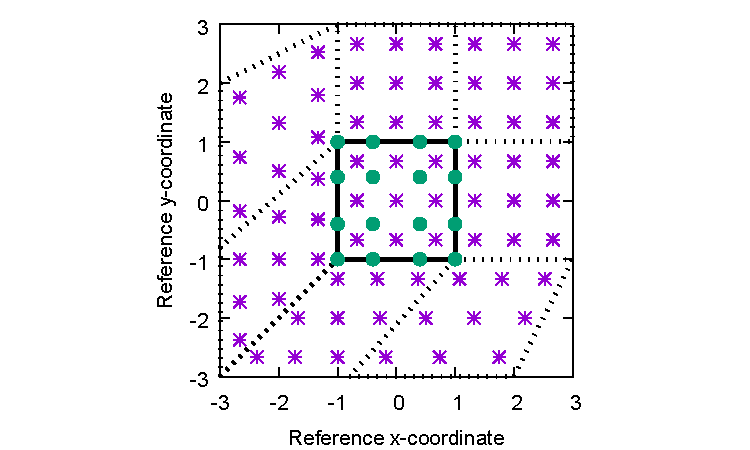
\includegraphics[width=19pc,angle=0]{figs/mapping/mapping.pdf}\\
\caption{}
\label{fig:mapping}
\end{figure}

%\appendix

% Use \appendix[A], \appendix}[B], if you have multiple appendixes.
%\appendix[A]

%% Appendix title is necessary! For appendix title:
%\appendixtitle{}

%%% Appendix section numbering (note, skip \section and begin with \subsection)
% \subsection{First primary heading}

% \subsubsection{First secondary heading}

% \paragraph{First tertiary heading}

%% Important!
%\appendcaption{<appendix letter and number>}{<caption>} 
%must be used for figures and tables in appendixes, e.g.,
%
%\begin{figure}
%\noindent\includegraphics[width=19pc,angle=0]{figure01.pdf}\\
%\appendcaption{A1}{Caption here.}
%\end{figure}
%
% All appendix figures/tables should be placed in order AFTER the main figures/tables, i.e., tables, appendix tables, figures, appendix figures.
%
%%%%%%%%%%%%%%%%%%%%%%%%%%%%%%%%%%%%%%%%%%%%%%%%%%%%%%%%%%%%%%%%%%%%%
% REFERENCES
%%%%%%%%%%%%%%%%%%%%%%%%%%%%%%%%%%%%%%%%%%%%%%%%%%%%%%%%%%%%%%%%%%%%%
% Make your BibTeX bibliography by using these commands:
\bibliographystyle{ametsoc2014}
\bibliography{bib}


%%%%%%%%%%%%%%%%%%%%%%%%%%%%%%%%%%%%%%%%%%%%%%%%%%%%%%%%%%%%%%%%%%%%%
% TABLES
%%%%%%%%%%%%%%%%%%%%%%%%%%%%%%%%%%%%%%%%%%%%%%%%%%%%%%%%%%%%%%%%%%%%%
%% Enter tables at the end of the document, before figures.
%%
%
%\begin{table}[t]
%\caption{This is a sample table caption and table layout.  Enter as many tables as
%  necessary at the end of your manuscript. Table from Lorenz (1963).}\label{t1}
%\begin{center}
%\begin{tabular}{ccccrrcrc}
%\hline\hline
%$N$ & $X$ & $Y$ & $Z$\\
%\hline
% 0000 & 0000 & 0010 & 0000 \\
% 0005 & 0004 & 0012 & 0000 \\
% 0010 & 0009 & 0020 & 0000 \\
% 0015 & 0016 & 0036 & 0002 \\
% 0020 & 0030 & 0066 & 0007 \\
% 0025 & 0054 & 0115 & 0024 \\
%\hline
%\end{tabular}
%\end{center}
%\end{table}

%%%%%%%%%%%%%%%%%%%%%%%%%%%%%%%%%%%%%%%%%%%%%%%%%%%%%%%%%%%%%%%%%%%%%
% FIGURES
%%%%%%%%%%%%%%%%%%%%%%%%%%%%%%%%%%%%%%%%%%%%%%%%%%%%%%%%%%%%%%%%%%%%%
%% Enter figures at the end of the document, after tables.
%%
%
%\begin{figure}[t]
%  \noindent\includegraphics[width=19pc,angle=0]{figure01.pdf}\\
%  \caption{Enter the caption for your figure here.  Repeat as
%  necessary for each of your figures. Figure from \protect\cite{Knutti2008}.}\label{f1}
%\end{figure}

\end{document}
